\documentclass[11pt, oneside]{article} 
\usepackage{geometry}
\geometry{letterpaper} 
\usepackage{graphicx}
	
\usepackage{amssymb}
\usepackage{amsmath}
\usepackage{parskip}
\usepackage{color}
\usepackage{hyperref}

\graphicspath{{/Users/telliott_admin/Tex/png/}}
% \begin{center} 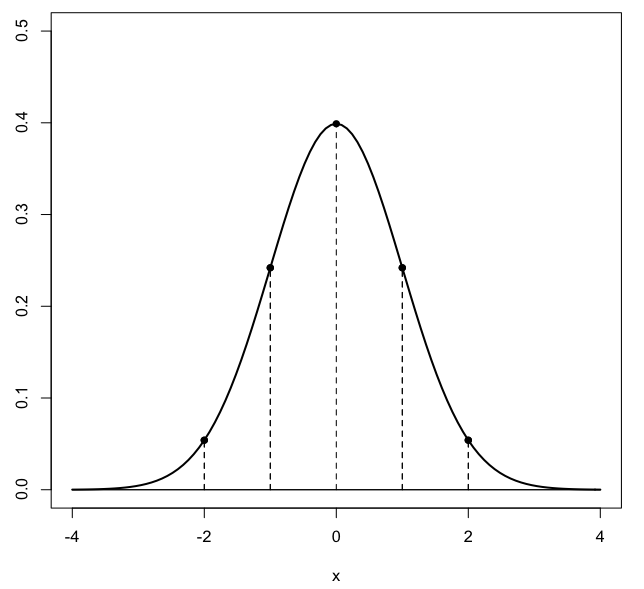
\includegraphics [scale=0.4] {gauss3.png} \end{center}

\title{Parabola}
\date{}

\begin{document}
\maketitle
\Large
\label{sec:Parabola_geometry}
You probably know that the \emph{conic sections} are the parabola, circle and ellipse, and hyperbola.
\begin{center} 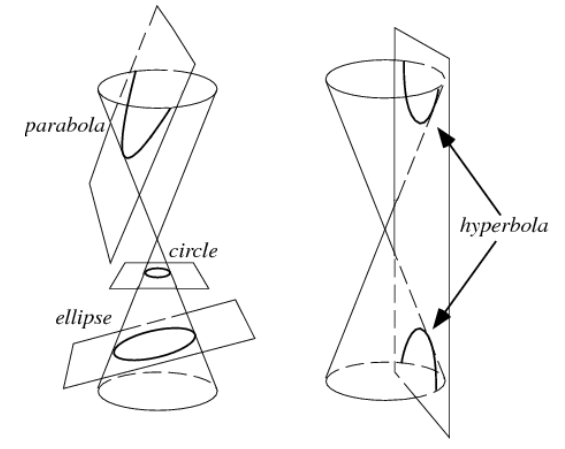
\includegraphics [scale=0.5] {conic_sections.png} \end{center}

After the circle, perhaps the most familiar of these is the parabola.  Consider a parabola in standard orientation, opening up and with its axis of symmetry pointed straight up and down.
\begin{center} 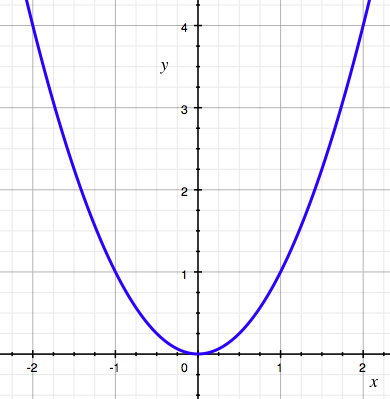
\includegraphics [scale=0.4] {para5.png} \end{center}

A parabola of this orientation whose vertex is located at the origin and with axis of symmetry $x=0$ is described by the very simple equation
\[ y = ax^2 \]
For the one shown above, $a$ is equal to $1$, giving $y = x^2$.  For example, the points $(1,1)$ and $(2,4)$ lie on the curve.

\subsection*{polynomials and quadratics}

A \textbf{polynomial} is a sum containing various powers of an independent variable, which is usually given as $x$.  For example:
\[ y = c_4 x^4 + c_3 x^3 + c_2 x^2 + c_1 x + c_0 \]

The powers must be positive integers or zero:  $n \in \{ 0, 1, 2 \dots \}$.

Each power $x^n$ is multiplied by its corresponding constant $c_n$.  The original equation might contain multiple coefficients for a given power $x^n$ that are then combined to form the constant.  

Each $c_n$ is some real number.  It is usual in examples for these constants to be integers, but this is by no means a requirement.

A \textbf{quadratic} is a polynomial that contains a term with $x^2$ but no higher powers of $x$:
\[ y = c_2 x^2 + c_1 x + c_0 \]
This is usually written as
\[ y = ax^2 + bx + c \]
where $a,b,$ and $c$ are constants.

A quadratic may or may not contain lower powers of $x$.  That is, either or both of $b$ and $c$ might be equal to zero.  All of these are quadratics:
\[ y = ax^2 \]
\[ y = ax^2 + bx \]
\[ y = ax^2 + c \]

In general, the roles the constants $a$ and $c$ play in the graph of a quadratic are fairly obvious, while that of $b$ is more subtle.  

Changing the value of $c$ shifts the graph up or down by the amount added.  Comparing
\[ y = ax^2 \]
\[ y = ax^2 + c \]
the second graph will be identical to the first, simply shifted up by $c$.

\subsection*{shape factor}

$a$ is called the \textbf{shape factor}.  If $a$ is positive, then the two "arms" of the parabola open up, and the \textbf{vertex} is the minimum value of the graph of the function.  

\begin{center} 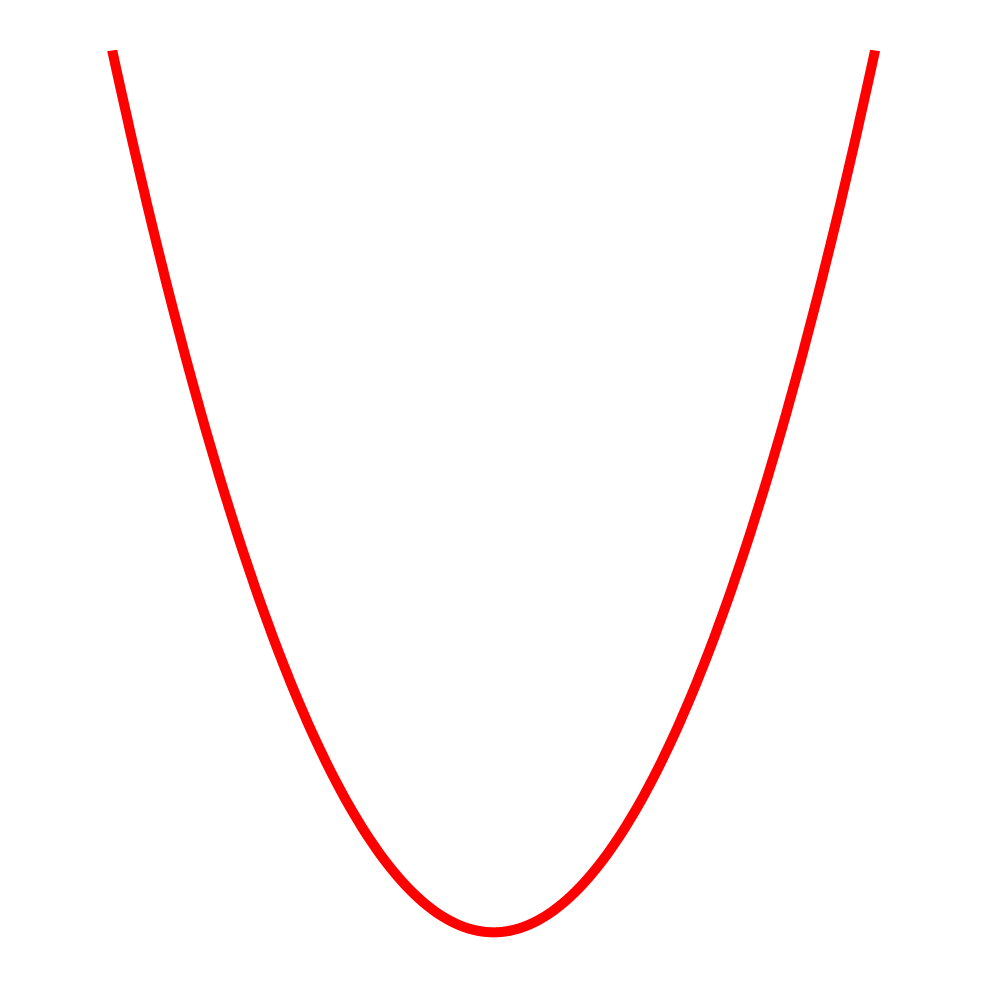
\includegraphics [scale=0.1] {para4.png} \end{center}
If $a$ is negative, then the graph opens down, and the vertex is the maximum.
\begin{center} 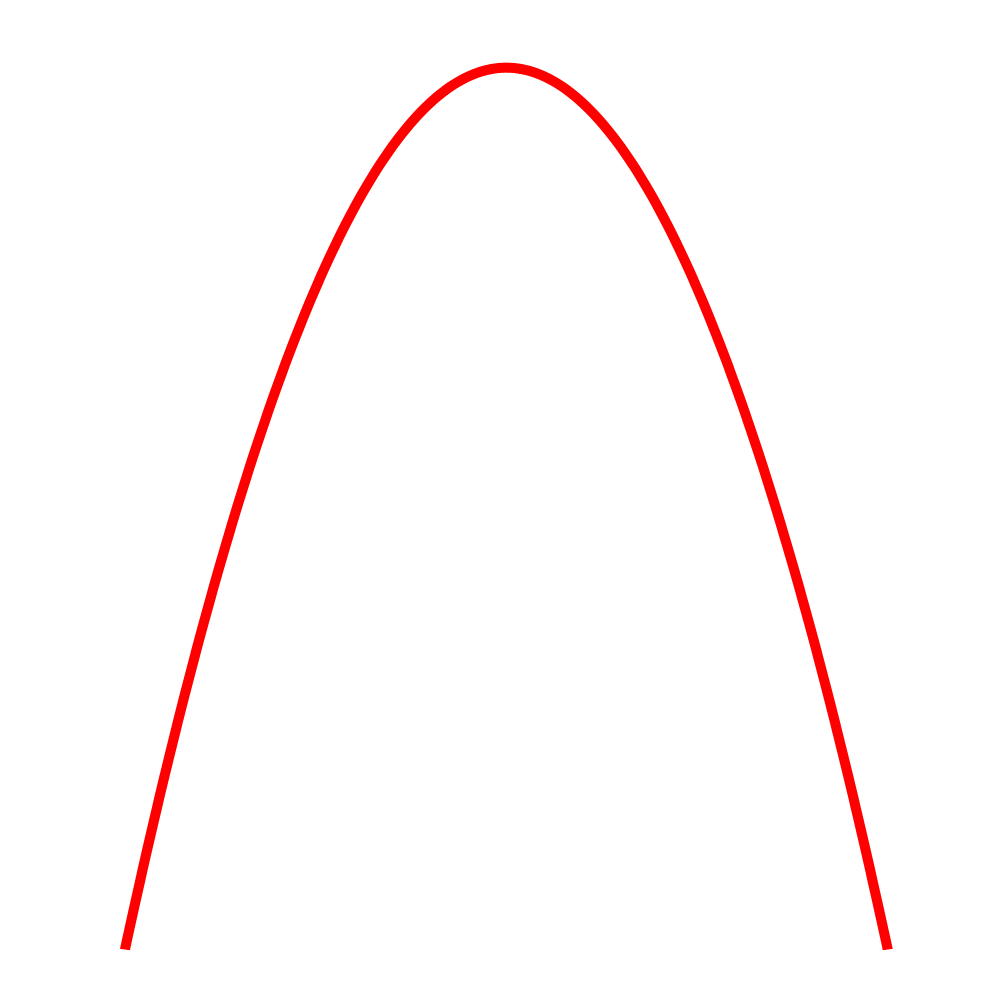
\includegraphics [scale=0.1] {para6.png} \end{center}

Any quadratic is symmetrical about the vertical axis that goes through its minimum (or maximum) point, the vertex.  

For the rest of this discussion, we will only consider $a > 0$.   If $a < 0$, the whole graph is flipped upside down. In that case, everywhere I say "minimum", we have a maximum instead.

Suppose
\[ y = ax^2 \]
$x^2$ is always greater than or equal to zero ($x^2 \ge 0$), therefore so is the value of this function, $y \ge 0$.  The minimum value is the vertex at $(x=0,y=0)$.
\begin{center} 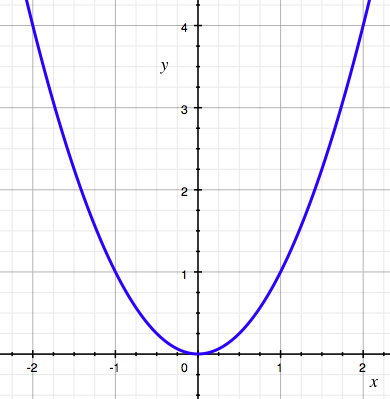
\includegraphics [scale=0.4] {para5.png} \end{center}

The graph is symmetrical about the $y$-axis.  This is also evident because $y = ax^2$ is an even function:  $f(x) = f(-x)$.

Consider the values of $y$ corresponding to $x = \{ 1, 2, 3, 4 \}$.  These are $y = \{ a, 4a, 9a, 16a \}$.  They increase like the square of $x$, but \emph{linearly} with $a$.  

If we plot $y = x^2$ and compare it to $y = 4x^2$, every $y$ value in the second plot can be taken from the first one, just multiplied by $4$.  $a$ stretches the plot linearly in the $y$-direction.

A substitution of variables $v = y/a$ turns $y = ax^2$ into $v = x^2$.
\subsection*{vertex}

Every parabola with the same value of $a$ has exactly the same shape.  For the same $a$, they may differ in the position of the vertex, depending on the other constants, $b$ and $c$.  The graph of a parabola depends only on the shape factor and the position of the vertex.

The coordinates at the vertex are usually given as constants $(h,k)$.  Suppose the vertex of the parabola is at $(h,k)$ with $a = 1$.  Then the equation of the parabola is
\[ (y - k) = (x - h)^2 \]
It may seem counterintuitive that we subtract the value of the variable at the vertex, but this is consistent across all of the conic sections.

Rearranging
\[ y = (x - h)^2 + k \]
we see that $y - k$ is like adding $k$ to the constant $c$, it moves the graph up the page.

Expand
\[ (y - k) = a(x - h)^2 \]
\[ y = ax^2 - 2ahx + h^2 + k \]
and compare with the canonical representation
\[ y = ax^2 + bx + c \]
The coefficients of corresponding powers must be equal so
\[ -2ah = b \]
\[ h = -\frac{b}{2a} \]

The $x$-value of the vertex is $x = -b/2a$.  Also
\[ h^2 + k = c \]
The $y$-value of the vertex is 
\[ k = c - h^2 = c - b^2/4a \]

\begin{center} 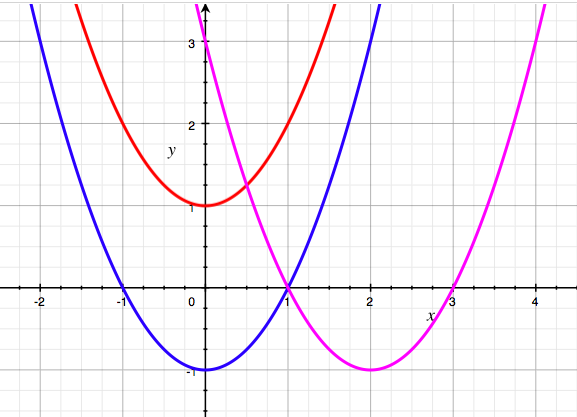
\includegraphics [scale=0.4] {para7.png} \end{center}
Here are three plots, all with shape factor $a = 1$, which differ only in the position of the vertex: $y = x^2 - 1$ (blue), $y = x^2 + 1$ (red), and $y = (x - 2)^2 - 1$ (magenta).

The two with the vertex below the $x$-axis have $c = -1$, while the one with the vertex above the $x$-axis has $c = 1$.

Notice that the magenta one has $h=2$.  To write it in  canonical form, expand 
\[ y = (x - h)^2 - 2 \]
\[ = x^2 - 2xh + h^2 - 2 \]
\[ = x^2 - 4x + 2 \]
Even though $c > 0$ for this one, the vertex is below the $x$-axis.  That's because $b = -2h$ also affects the placement of the vertex.  We see that effect here as $c = h^2 - 2$.

\subsection*{roots}
The roots of a quadratic are those values of $x$ for which the corresponding value of $y$ is  zero.  

For example, if $x = 0$ then
\[ y = x^2 = 0^2 = 0 \]

$x = 0$ is the only value that yields this result, since if $x \ne 0$, then $y = x^2 > 0$.

Suppose we shift the graph of the equation \emph{down}, by subtracting $1$, i.e. letting $c = -1$:
\[ y = x^2 - 1 \]
From examining the plot of this function you will observe that there are two points where the graph of the function crosses the $x$-axis (where $y = 0$).  We can guess them from the plot as $x = \pm 1$, and confirm that result directly by substituting into the equation and checking that we get $y = 0$.

\[ y =  (1)^2 - 1 = 0 \]
\[ y =  (-1)^2 - 1 = 0 \]

Another way to get this answer is to factor the original equation.
\[ y = (x + 1)(x - 1) \]

Now it is obvious that either $x = \pm 1$ gives $y = 0$ as the result.

If a quadratic can be factored to the form
\[ y = (x - r_1)(x - r_2) \]
then $r_1$ and $r_2$ are the roots, because if $x = r_1$ or $x = r_2$, then $y = 0$.

On the other hand, suppose we shift the graph \emph{up}
\[ y = x^2 + 1 \]
Since $x^2$ is always positive or zero, there is no value of $x$ which gives $y = 0$.  We say that such an equation has no (real) roots.  An equivalent statement or observation is that its graph does not cross the $x$-axis.

Again, if a quadratic can be factored to the form
\[ y = (x - r_1)(x - r_2) \]
then
\[ y = x^2 - (r_1 + r_2) x + r_1 r_2 \]
In the canonical representation
\[ ax^2 + bx + c \]
$c$ is the product of the roots, and $b$ is the negative of the sum.

For the example 
\[ y = x^2 - 1 \]
the sum of the roots is $0$ and their product is $-1$.  From the first fact:
\[ r_2 = - r_1 \]
substituting into the second.
\[ r_1^2 = 1 \]

If you've had practice factoring quadratics with integer roots, you should be very familiar with this fact:  $c$ is the product of the roots, and $b$ is the negative of the sum.

\subsection*{three types}
In summary, we can classify parabolas into three types.  

The first one has a graph that does not cross the $x$-axis.  It has no real roots.

The second type has a graph that does cross the $x$-axis and has two distinct real roots of the form
\[ y = (x - r_1)(x - r_2) \]

The third one has repeated roots
\[ y = (x - r)(x - r) \]
This type has a single value of $x$ that yields $y = 0$.  This happens when the graph of the parabola just touches the $x$-axis --- the vertex is on the $x$-axis.

The example given above $y = x^2$ is a special case of this type where $r = 0$.

\subsection*{quadratic formula}
The quadratic formula gives the roots of any quadratic.  In the case where there are no real roots, the results from the quadratic formula are complex numbers of the form $p \pm q \sqrt{-1}$, (where $p$ and $q$ are real numbers).

The formula is
\[ x = \frac{-b \pm \sqrt{b^2 - 4ac}}{2a} \]
You should memorize this.

Examples:

$y = x^2$
\[ x = \frac{-(0) \pm \sqrt{0^2 - 4(1)(0)}}{2(1)} = 0 \]

$y = x^2 - 1$
\[ x = \frac{-(0) \pm \sqrt{0^2 - 4(1)(-1)}}{2(1)} = \pm \frac{\sqrt{4}}{2} = \pm 1 \]

$y = x^2 + 1$
\[ x = \frac{-(0) \pm \sqrt{0^2 - 4(1)(1)}}{2(1)} =  \pm \frac{\sqrt{-4}}{2} = ?? \]

The result of the last calculation is a pair of complex numbers.  A complex number is a number of the form $p + q \sqrt{-1}$, often written $p + iq$.

We may write the expression under the square root as
\[ D = b^2 - 4ac \]
where $D$ stands for discriminant.  If $D < 0$ then the result is a pair of complex numbers and we say there are no real roots.  If $D = 0$ then there is a single (repeated) root.

Although the existence of complex roots means the graph does not cross the $x$-axis and there is no $x$ such that $f(x) = 0$, nevertheless these roots do have physical meaning.  

The two complex roots are related, they are called complex conjugates.  

Label them as $z = p \pm q \sqrt{-1}$ and plug them into the factored quadratic
\[ y = (x - z_1)(x - z_2) \]
\[ y = \ [ \ x - (p + q \sqrt{-1} ) \ ] \ [ \ x - (p - q \sqrt{-1} ) \ ] \]
\[ = (x - p - q \sqrt{-1})(x - p + q \sqrt{-1}) \]
Multiplying this out, the square roots will (always) disappear:
\[ y = x^2 - px + xq \sqrt{-1} - px + p^2 - pq \sqrt{-1} - xq \sqrt{-1} + pq \sqrt{-1} + q^2 \]
\[ = x^2 - 2px + p^2 + q^2 \]
\[ = (x - p)^2 + q^2 \]

The meaning of this is the following:  even with complex roots, the factored form gives a real result when multiplied out.  The real part of $z = p \pm q \sqrt{-1}$ is $p$, and this is the value of $x$ at the minimum.  

$q^2$ is the displacement of the vertex up from the $x$-axis at the minimum.

\subsection*{more about b}
Consider the basic equation
\[ y = ax^2 + bx + c \]
\[ \frac{y - c}{a} = x^2 + \frac{b}{a} x \]

By judicious manipulation we can make the last term $b/a \cdot x$ go away (this is  \emph{always} true).  The general procedure is called completing the square.  Write
\[ x^2 + \frac{b}{a} x + \_\_\_ = (x +  \_\_\_)^2 \]

We seek two values to substitute for the spaces $ \_\_\_$.  

Now, of course, the $\_\_\_$ on the left-hand side is the square of the second one, on the right.  

But there is another constraint.  Namely, the second $\_\_\_$ is related to the cofactor of $x$ on the left-hand side.

Recall that
\[ x^2 + 2mx + m^2 = (x + m)^2 \]
Compare that with 
\[ x^2 + \frac{b}{a} x + \_\_\_ = (x +  \_\_\_)^2 \]
Can you see that $b/a$ must be equal to $2m$ and so $m = b/2a$?  We need two copies of the second term in the binomial expansion ($m$), to put as the cofactor of $x$ in the term $2mx$.  Since the standard form in the last expression has $b/a$ equivalent to $2m$, we get $b/2a$ equivalent to $m$.

If that's not clear, just verify that the following works.  Write:
\[ x^2 + \frac{b}{a} x + \_\_\_ = (x +  \frac{b}{2a})^2 \]
\[ x^2 + \frac{b}{a} x + (\frac{b}{2a})^2 = (x +  \frac{b}{2a})^2 \]

Now that we know what is needed to complete the square, go back to our problem.
\[ \frac{y - c}{a} = x^2 + \frac{b}{a} x \]

To make the perfect square, we add $(b/2a)^2$ to the right-hand side, and to maintain the equality add the same thing to the left-hand side:
\[ \frac{y - c}{a} +  (\frac{b}{2a})^2 = x^2 + \frac{b}{a} x +  (\frac{b}{2a})^2 \]

As we saw above, the right-hand side is also $(x + b/2a)^2$ so we can write
\[ \frac{y - c}{a} +  (\frac{b}{2a})^2 = (x +  \frac{b}{2a})^2 \]
Finally, multiply through by $a$ and rearrange slightly
\[ y = a(x +  \frac{b}{2a})^2 + c - \frac{b^2}{4a}  \]

We can get several things from this.  

First, the minimum value of $y$ occurs when the squared term is equal to zero, that is when
\[ x +  \frac{b}{2a} = 0 \]
\[ x = - \frac{b}{2a} \]
Therefore, the vertex of the parabola is at this value of $x$.  We found this earlier by writing $(y - k) = a(x - h)^2$ and multiplying out.

When $x = -b/2a$, the corresponding value of $y$ is
\[ y = a(-\frac{b}{2a} +  \frac{b}{2a})^2 + c - \frac{b^2}{4a} \]
\[ = c - \frac{b^2}{4a}  \]
This also matches what we had before.
 
Second and more generally, the roots occur when
\[ y = 0 = a(x +  \frac{b}{2a})^2 + c - \frac{b^2}{4a}  \]
\[ a(x + \frac{b}{2a})^2 = \frac{b^2}{4a} - c  \]
\[ (x + \frac{b}{2a})^2 = \frac{b^2-4ac}{4a^2}  \]
\[ x + \frac{b}{2a} = \pm \frac{\sqrt{b^2-4ac}}{2a}  \]
\[ x = \frac{-b \pm \sqrt{b^2-4ac}}{2a}  \]
which is the quadratic formula.

Third, any quadratic can be rewritten as
\[ y = a(x +  \frac{b}{2a})^2 + c - \frac{b^2}{4a}  \]
\[ y = a(x-h)^2 + k \]

\subsection*{translation}
The basic shape depends only on $a$.  

$b$ (combined with $2a$) moves the vertex right or left from the $y$-axis.

$a,b,c$ all together combine to move it up and down from the $x$-axis.  

If you play around with a plotting application and change $b$ you will find that the shape stays the same, but both the $x$ and the $y$-values of the vertex will change as $b$ changes.

Here are the three plots again. 
\begin{center} 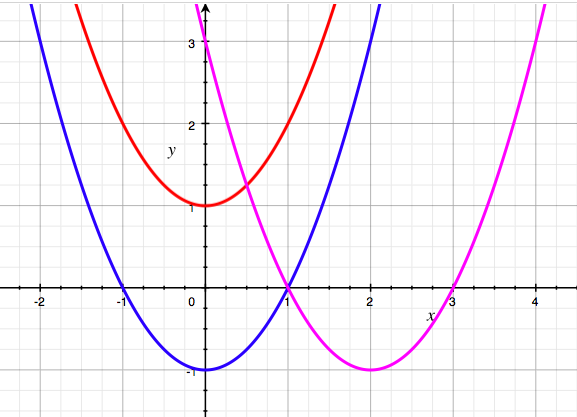
\includegraphics [scale=0.4] {para7.png} \end{center}
$y = x^2 - 1$ (blue), $y = x^2 + 1$ (red), and $y = (x - 2)^2 - 1$ (magenta).

The two with the vertex on the $y$-axis have $h = 0$, the other has $h = 2$.  

The plots with real roots have $k = -1$ and $(y - k) = y + 1$, the other has $k = 1$.

For example, the lower right-hand plot is
\[ (y + 1) = (x - 2)^2 = x^2 - 4x + 4 \]
\[ y = x^2 - 4x + 3 \]

This can be factored easily:
\[ y = (x - 1)(x - 3) \]
The roots are at $x = 1, x = 3$, which checks.

\subsection*{rotation}
You might ask, what about rotation?  For example, if we rotate $y = x^2$ by $45$ degrees clockwise, what would be the equation to describe it?  The short answer is that such equations do exist, and they have terms like $xy$ or $uv$ in them.  They are not polynomials of the type we've been describing.

As an example to rotate through $45^\circ$, replace $x$ and $y$ by $u$ and $v$ with
\[ x = u \cos \theta - v \sin \theta = \frac{u}{\sqrt{2}} - \frac{v}{\sqrt{2}} \]
\[ x = ku - kv \]

\[ y = u \sin \theta + v \cos \theta = \frac{u}{\sqrt{2}} + \frac{v}{\sqrt{2}} \]
\[ y = ku + kv \]

Substitute for $x$ and $y$ in the standard equation:
\[ y = ax^2 + bx + c \]

\[ ku + kv = a(ku - kv)^2 + b(ku - kv) + c \]
\[ u + v = ak(u^2 - 2uv + v^2) + b(u - v) + \frac{c}{k} \]
Notice the term $-2akuv$ that mixes $u$ and $v$.  

This is a more advanced topic than we can deal with here.

\subsection*{focus and directrix}
There is a geometric definition of the parabola.  Based on what we said above, without loss of generality, we can translate any parabola to the origin of coordinates, with equation $y = ax^2$.

Now, pick a point on the $y$-axis a distance $p$ up from the origin, colored magenta in the figure.  This point is called the focus.

Then draw a line parallel to the $x$-axis which intersects the $y$-axis the same distance $p$ below the origin.  This line is called the directrix.  It is colored red and is dashed.

\begin{center} 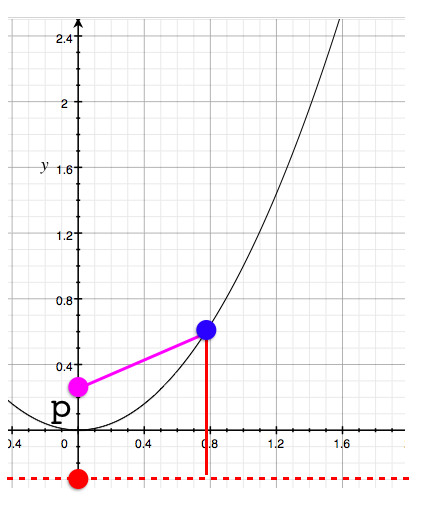
\includegraphics [scale=0.4] {focus_dir.png} \end{center}
The parabola consists of all those points whose distance to the focus is equal to the vertical distance to the directrix.

Pick an arbitrary point on the parabola (in blue), with coordinates $(x, ax^2)$.  The squared distance to the focus (magenta point) is 
\[ \Delta y^2 + \Delta x^2 = (ax^2 - p)^2 + x^2 \]

while the squared distance to the directrix (red line) is  $(ax^2 + p)^2$.  

For the correct choice of $p$ these distances are to be equal:
\[ (ax^2 - p)^2 + x^2 = (ax^2 + p)^2 \]
\[ a^2 x^4 - 2ap x^2 + p^2 + x^2 = a^2x^4 + 2apx^2 + p^2 \]

Canceling two terms on each side
\[ - 2ap x^2 + x^2 =  + 2apx^2  \]
Divide by $x^2$
\[ - 2ap + 1 =  2ap  \]
\[ 4ap = 1 \]
\[ p = \frac{1}{4a} \]

The shape factor $a$ determines the distance of the focus from the origin, which is $p$, and from the directrix, which is $2p$.

\end{document} 